\documentclass[11pt]{article}
\usepackage[margin=0.72in]{geometry}
\usepackage{array,booktabs,enumitem,graphicx,multicol,xcolor}
\usepackage{amsmath,amssymb}
\usepackage{listings}
\usepackage{tikz}
\usepackage[american]{circuitikz}
\usetikzlibrary{arrows.meta,positioning}
\graphicspath{{docs/lessons/assets/}{../assets/}}
\setlength{\parindent}{0pt}
\setlength{\parskip}{5pt}
\setlist{nosep}
\definecolor{codebg}{RGB}{246,246,242}
\definecolor{ruleblue}{RGB}{35,75,115}
\lstset{language=C++,basicstyle=\ttfamily\small,backgroundcolor=\color{codebg},
  frame=single,breaklines=true,showstringspaces=false,columns=fullflexible}
\newcommand{\checkblank}{\(\square\)}
\newcommand{\state}[1]{\textbf{State #1}}
\newcommand{\evidence}{\textbf{Evidence: }}

\begin{document}

\begin{center}
{\LARGE\bfseries Lesson 003: One Package, Three LEDs}\\[3pt]
{\large Common-cathode RGB color mixing with PWM --- Arduino Mega 2560}\\
\end{center}

\begin{tabular}{@{}p{0.48\linewidth}p{0.48\linewidth}@{}}
\textbf{Name:} \hrulefill & \textbf{Date / team:} \hrulefill\\[6pt]
\textbf{Board ID:} \hrulefill & \textbf{Observer:} \hrulefill
\end{tabular}

\section*{The question}
How can three independently controlled LED dice inside one package make colors that
appear continuous, and what evidence distinguishes PWM mixing from simply switching
three LEDs on or off?

\textbf{Learning targets.} By the end, you can (1) identify common cathode and the
three anodes, (2) protect \emph{each} channel with its own resistor, (3) predict and
measure RGB PWM duty behavior, (4) explain why duty cycle and PWM frequency are
different quantities, and (5) explain the planned C++ composition and RAII lifecycle.

\section*{Safety gate --- complete before applying USB power}
\begin{itemize}
  \item \checkblank{} Disconnect USB power while building or moving wires.
  \item \checkblank{} Use a \textbf{common-cathode} RGB LED. Confirm its datasheet
        pinout; package lead order is not universal.
  \item \checkblank{} Connect the common cathode only to Mega GND.
  \item \checkblank{} Install \textbf{exactly one series resistor per color channel}
        (three resistors total). Never share one resistor on the common lead.
  \item \checkblank{} Inspect for a 5\,V--GND short and for adjacent legs touching.
  \item \checkblank{} Power down immediately for heat, odor, flicker unrelated to the
        program, or a reset loop.
\end{itemize}
\textbf{Current budget.} Prefer 330\(\Omega\) on every channel. We design for modest
indicator current, not maximum brightness. Do not infer safe current from ``it still
lights.'' Before use, check both each pin's current and the aggregate current against
the \emph{official ATmega2560 and board documentation}; a per-pin maximum is not a
design target, and timer-port/package aggregate limits still apply.

\section*{Concept first, wiring second}
\begin{center}
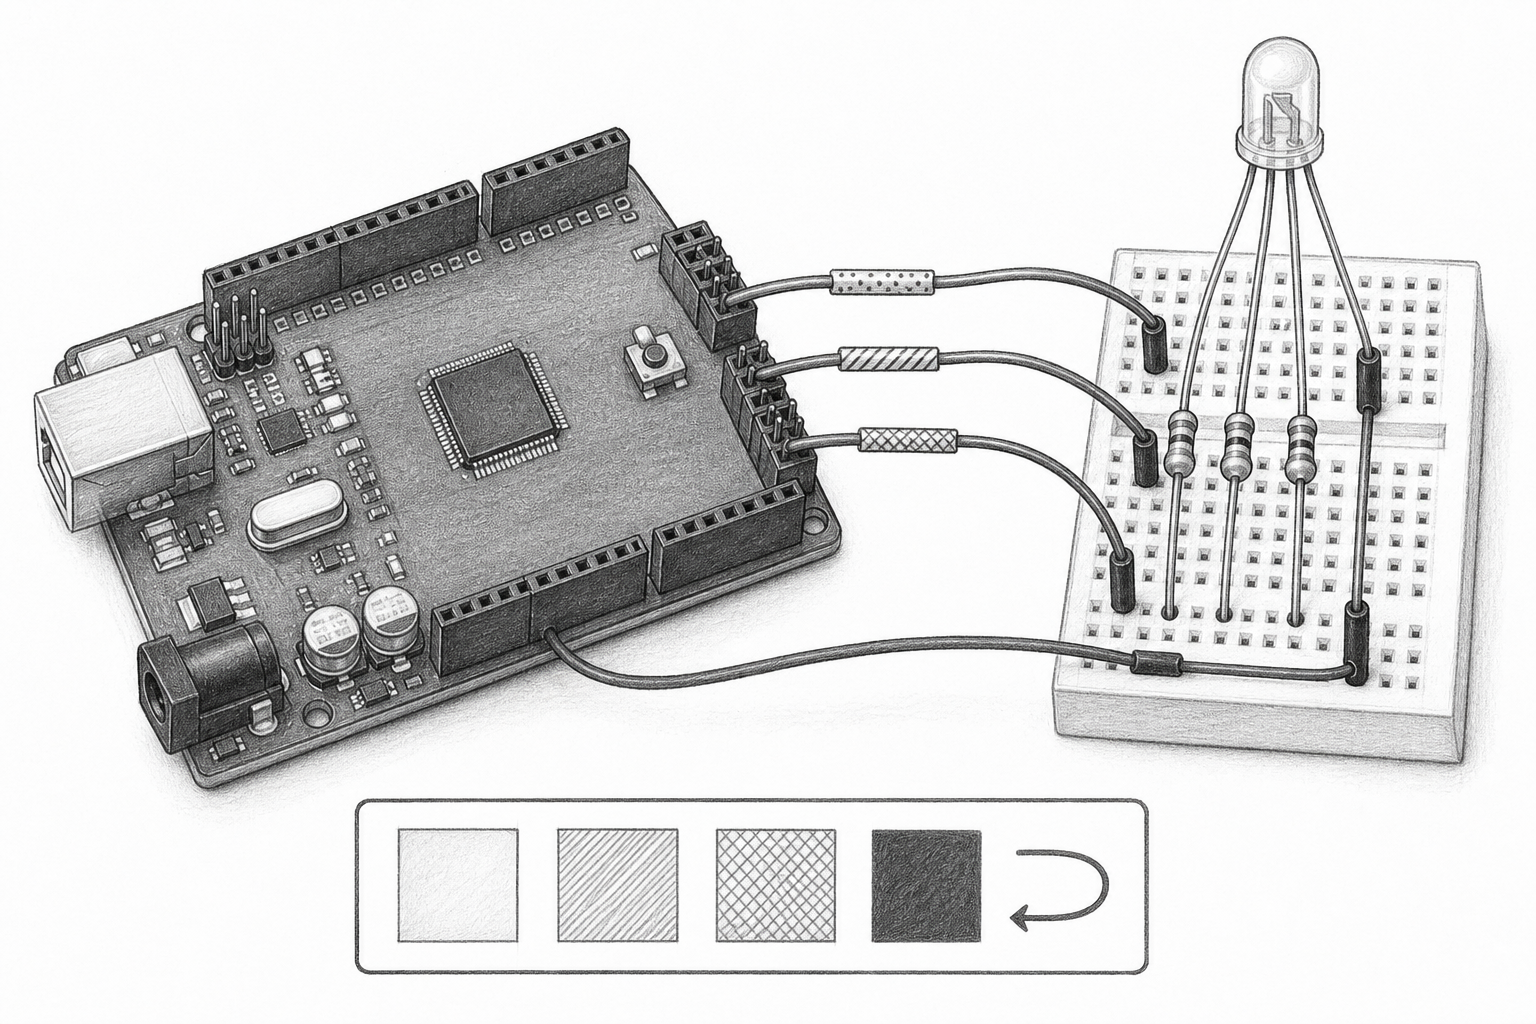
\includegraphics[width=0.76\linewidth]{003-rgb-led-pencil.png}
\end{center}
\textit{Figure 1 is a conceptual pencil drawing. It communicates the idea of mixed
light; it is not an authoritative pin-by-pin wiring diagram. Build only from
Figure 2 and the LED manufacturer's pinout.}

\section*{Exact electrical schematic}
\begin{center}
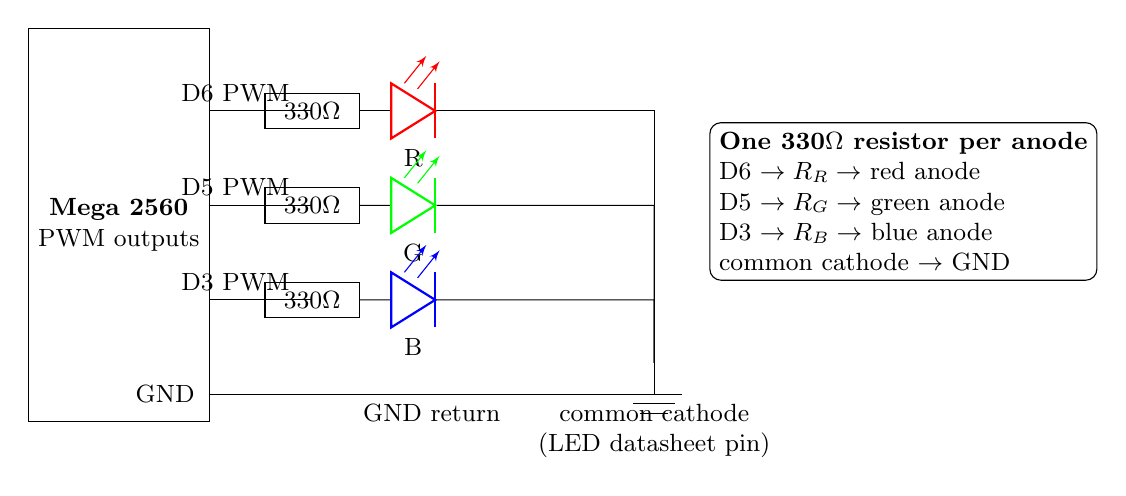
\begin{tikzpicture}[x=1cm,y=1cm,>=Latex,font=\small]
  \node[draw,minimum width=2.3cm,minimum height=5.0cm,align=center] (mega) at (0,0)
       {\textbf{Mega 2560}\\PWM outputs};
  \coordinate (p6) at (mega.east |- 0,1.45);
  \coordinate (p5) at (mega.east |- 0,0.25);
  \coordinate (p3) at (mega.east |- 0,-0.95);
  \draw (p6) -- ++(0.65,0) node[above,midway]{D6 PWM} -- ++(0.65,0)
        node[draw,minimum width=1.2cm,minimum height=.42cm] (rr) {330\(\Omega\)};
  \draw (p5) -- ++(0.65,0) node[above,midway]{D5 PWM} -- ++(0.65,0)
        node[draw,minimum width=1.2cm,minimum height=.42cm] (rg) {330\(\Omega\)};
  \draw (p3) -- ++(0.65,0) node[above,midway]{D3 PWM} -- ++(0.65,0)
        node[draw,minimum width=1.2cm,minimum height=.42cm] (rb) {330\(\Omega\)};
  \foreach \r/\yy/\c/\lab in {rr/1.45/red/R,rg/.25/green/G,rb/-.95/blue/B}
  {
    \draw (\r.east) to[leD,l_=\lab,color=\c] ++(1.35,0)
          -- (6.8,\yy) -- (6.8,-1.75);
  }
  \draw (6.8,-1.75) -- (6.8,-2.15)
        node[below,align=center]{common cathode\\(LED datasheet pin)};
  \draw (6.8,-2.15) -- (1.15,-2.15) node[midway,below]{GND return};
  \draw (1.15,-2.15) -- (mega.east |- 0,-2.15);
  \node[left=2pt] at (mega.east |- 0,-2.15) {GND};
  \draw (6.45,-2.15) -- (7.15,-2.15);
  \draw (6.53,-2.27) -- (7.07,-2.27);
  \draw (6.62,-2.39) -- (6.98,-2.39);
  \node[draw,rounded corners,align=left,anchor=west] at (7.5,.3)
       {\textbf{One 330\(\Omega\) resistor per anode}\\
        D6 \(\rightarrow R_R \rightarrow\) red anode\\
        D5 \(\rightarrow R_G \rightarrow\) green anode\\
        D3 \(\rightarrow R_B \rightarrow\) blue anode\\
        common cathode \(\rightarrow\) GND};
\end{tikzpicture}
\end{center}

\textbf{Polarity caveat.} This circuit is common-cathode, so larger PWM values mean
more on-time and usually more light. A common-anode part reverses the logic and
cannot be substituted without changing both wiring and software. PWM is rapid
digital switching, \emph{not} a true analog voltage. Values 0 and 255 are intended
as the off and fully-on endpoints, but exact endpoint behavior is core- and
timer-dependent. The high level under load is \(V_{OH}\), not an assumed ideal
5.000\,V; it falls as source current rises. Pins 6, 5, and 3 are selected
because they support hardware PWM on the Mega 2560; timer configuration by other
libraries can change PWM frequency or availability.

\section*{Prediction before construction}
Assume \texttt{on(Color)} maps an 8-bit channel value \(x\) to a duty cycle
\[
       D=\frac{x}{255}\times100\%.
\]
Predict before testing; use words such as dark, dim, medium, bright, or a color name.

\begin{center}
\begin{tabular}{@{}lrrrrp{3.0cm}@{}}
\toprule
Command & R & G & B & predicted duty pattern & predicted appearance\\
\midrule
red    & 255&0&0& R 100\%, others 0\% & \\
green  & 0&255&0& G 100\%, others 0\% & \\
blue   & 0&0&255& B 100\%, others 0\% & \\
orange & \rule{.8cm}{.2pt}&\rule{.8cm}{.2pt}&0&
        \rule{2.8cm}{.2pt}&\rule{2.8cm}{.2pt}\\
\bottomrule
\end{tabular}
\end{center}

\textbf{Prediction claim:} If red and green PWM are both active, then I predict
\rule{3cm}{.2pt}, because \rule{7cm}{.2pt}.

\newpage
\section*{Setup and controlled state sequence}
\textbf{Equipment:} Mega 2560, verified common-cathode RGB LED, three equal
330\(\Omega\) resistors, breadboard, jumpers, USB cable, and optionally a
multimeter or phone slow-motion camera.

\begin{enumerate}
  \item \state{0 --- powerless inspection.} USB disconnected. Identify pins from the
        LED datasheet. Build Figure 2. Record resistor markings or measured values.
  \item \state{1 --- isolation test.} Keep two anode jumpers disconnected. Connect
        one channel at a time and run only its primary color. Repeat R, G, B.
  \item \state{2 --- composed output.} Connect all three channels. Run the supplied
        Lesson 003 sequence: red, green, blue, orange, 250\,ms each.
  \item \state{3 --- controlled comparison.} Make this explicit temporary sketch
        change: add
        \texttt{const auto halfRed = adk::color::Rgb(128, 0, 0);} beside the other
        colors, then add \texttt{led.on (halfRed); delay(intervalMs);} immediately
        after full red. This uses the supplied library's public constructor and
        changes no library implementation. Keep pin, resistor, viewing position,
        room light, interval, and observation method fixed.
  \item \state{4 --- frequency evidence (instrument optional).} With an oscilloscope
        or logic analyzer, measure period \(T\) on D6 at red value 128 and calculate
        \(f=1/T\). Then measure at 255. Duty should change; frequency may be
        unmeasurable at the fully-on endpoint because there are no transitions.
        Without such an instrument, record ``not measured'' rather than treating
        camera bands or appearance as a frequency measurement.
  \item \state{5 --- power-down.} Disconnect USB before rewiring. This firmware does
        not yet supply a component-level lifecycle experiment.
\end{enumerate}

\section*{Record repeated evidence}
Do not use one glance as proof. Complete at least three cycles. ``Observed'' should
describe what happened, not what was expected.

\begin{center}
\small
\begin{tabular}{@{}clp{2.7cm}p{2.8cm}p{2.8cm}p{2.5cm}@{}}
\toprule
Trial & command & observed color & flicker/transition & unexpected behavior &
instrument evidence\\
\midrule
1 & R/G/B/orange & & & &\\[8mm]
2 & R/G/B/orange & & & &\\[8mm]
3 & R/G/B/orange & & & &\\[8mm]
\bottomrule
\end{tabular}
\end{center}

\begin{center}
\begin{tabular}{@{}lrrrp{4.2cm}@{}}
\toprule
D6 command & measured \(T\) & calculated \(f\) & measured duty & interpretation\\
\midrule
128 &&&&\\[6mm]
255 &&&&\\[6mm]
\bottomrule
\end{tabular}
\end{center}

\begin{center}
\begin{tabular}{@{}p{3.1cm}p{2.1cm}p{2.2cm}p{3.0cm}p{3.0cm}@{}}
\toprule
Controlled comparison & PWM value & predicted duty & measured or observed result &
constants held\\
\midrule
Full red & 255 & 100\% &&\\[7mm]
Half red & 128 & \rule{1.5cm}{.2pt} &&\\[7mm]
\bottomrule
\end{tabular}
\end{center}

\textbf{Required calculation.} Show the half-red duty calculation:
\[
 D=\frac{\rule{1.3cm}{.2pt}}{255}\times100\%
   =\rule{1.8cm}{.2pt}\%.
\]
If a multimeter reports average pin voltage, a rough ideal model is
\(V_{\rm avg}\approx D\times5.0\,\mathrm{V}\). Predict half-red:
\rule{2cm}{.2pt}\,V.

Explain why LED brightness is not necessarily half:\\[2mm]
\rule{\linewidth}{.2pt}

\newpage
\section*{Current-limiting calculation}
For each die, estimate
\[
 I_{\rm on}=\frac{V_{OH}-V_f}{R}.
\]
Use the LED datasheet \(V_f\), not a color-name guess, and use a measured loaded
\(V_{OH}\) or a conservative value justified from the MCU datasheet. Example only:
if measured \(V_{OH}=4.8\) V, red \(V_f=2.0\) V, and \(R=330\,\Omega\), then
\(I_{\rm on}=(4.8-2.0)/330=8.5\) mA. At 50\% duty, the simplified channel average
is about 4.2 mA. Repeat for the actual parts, then sum the worst simultaneous
channel currents and compare that aggregate with every applicable documented limit:

\begin{center}
\begin{tabular}{@{}lrrrr@{}}
\toprule
channel & measured \(R\) & datasheet \(V_f\) & calculated \(I_{\rm on}\) &
at tested duty, \(I_{\rm avg}\)\\
\midrule
red   &&&&\\[6mm]
green &&&&\\[6mm]
blue  &&&&\\[6mm]
\bottomrule
\end{tabular}
\end{center}
\[
 I_{\rm aggregate,worst}=I_R+I_G+I_B
 =\rule{2.0cm}{.2pt}\ {\rm mA}.
\]

\section*{The program and the object model}
\begin{lstlisting}
#include <adk.h>

adk::led::Rgb led(6, 5, 3);

const auto red    = adk::color::red();
const auto green  = adk::color::green();
const auto blue   = adk::color::blue();
const auto orange = adk::color::orange();

void setup()
{
    adk::initialize();
}

void loop()
{
    constexpr auto intervalMs = 250;

    led.on (red);    delay(intervalMs);
    led.on (green);  delay(intervalMs);
    led.on (blue);   delay(intervalMs);
    led.on (orange); delay(intervalMs);
}
\end{lstlisting}

\textbf{Composition.} An RGB LED is not a special kind of one-pin LED. It
\emph{has three} independently driven channels, so composition models the circuit:
an \texttt{Rgb} object owns or contains red, green, and blue output state. A
\texttt{Color} value describes desired intensities; it does not own pins.

\textbf{Planned lifecycle, not a claim about this firmware.} The current example
constructs a global \texttt{Rgb} and calls the library-level
\texttt{adk::initialize()}; it does not demonstrate per-component
\texttt{initialize()}, \texttt{shutdown()}, pin claiming, or destructor-driven
hardware cleanup. The target design is for explicit component
\texttt{initialize()} to acquire/configure transactionally, for idempotent
\texttt{shutdown() noexcept} to return outputs to their documented safe state, and
for the destructor to invoke that cleanup. In an exception-enabled host, ordinary
stack unwinding would then invoke destructors. These are interface requirements to
implement and test, not evidence supplied by this circuit. Copying a future
pin-owning object should be prohibited so ownership cannot be duplicated.

\textbf{Why code lives out of line.} Headers should expose the small contract while
implementation belongs in \texttt{.cpp} files. This reduces dependencies and rebuild
cost, avoids accidental code duplication, and lets the linker discard unused
features. Templates or genuinely compile-time operations are exceptions, not the
default.

\section*{Interpretation caveats}
\begin{itemize}
  \item Equal numeric R, G, and B values do not guarantee equal perceived brightness.
        LED efficiency, forward voltage, package optics, and human vision differ.
  \item A camera may show bands because its shutter samples PWM. That is evidence of
        switching and sampling, not necessarily visible flicker.
  \item \texttt{delay()} makes this demonstration simple but blocks input handling.
        Later components should use time-based updates so buttons can remain responsive.
  \item Apparent orange is additive light mixing. It is not evidence that photons
        themselves became ``orange paint.''
\end{itemize}

\section*{Troubleshooting by symptom}
\begin{tabular}{@{}p{0.25\linewidth}p{0.34\linewidth}p{0.35\linewidth}@{}}
\toprule
Symptom & likely cause & discriminating test (power off before rewiring)\\
\midrule
Nothing lights & wrong common pin, common-anode part, no ground, or no upload &
Verify datasheet and continuity; run one isolated channel.\\
One color missing & wrong LED lead, open jumper/resistor, damaged die, wrong pin &
Swap only the signal source between a known-good channel and failed channel.\\
Colors are permuted & anodes assigned to different physical dice &
Run isolation State 1 and label each lead from evidence.\\
Very bright / board resets & missing or bypassed resistor; short circuit &
Disconnect immediately; count three distinct series resistors and inspect rails.\\
Only primary colors work & mixed-color values or mapping is wrong &
Command two known nonzero channels and observe each separately first.\\
Unexpected inversion & common-anode device or inverted driver assumption &
Check common lead polarity with datasheet; do not ``fix'' by guessing.\\
Camera bands & camera shutter interacting with PWM &
Compare direct observation and two frame-rate settings.\\
\bottomrule
\end{tabular}

\section*{Assessment}
\begin{enumerate}
  \item Why is one resistor in the common cathode lead not equivalent to three
        resistors? \vspace{1.0cm}
  \item With PWM value 64, calculate ideal duty cycle. \vspace{0.8cm}
  \item Which single variable changed in State 3? Name two controlled variables.
        \vspace{0.8cm}
  \item Explain why \texttt{Rgb} should compose channels rather than inherit from
        one channel. \vspace{0.9cm}
  \item Which lifecycle behavior is present in today's sketch, and which behavior is
        only a target requirement?
        \vspace{0.8cm}
  \item A color is wrong. Propose a test that distinguishes software channel mapping
        from a failed LED die. \vspace{1.0cm}
\end{enumerate}

\section*{CER exit ticket}
\textbf{Claim.} State what the repeated trials show about PWM color mixing.\\
\rule{\linewidth}{.2pt}\\[7mm]
\textbf{Evidence.} Cite at least two specific observations or measurements, including
the controlled comparison.\\
\rule{\linewidth}{.2pt}\\[7mm]
\rule{\linewidth}{.2pt}\\[7mm]
\textbf{Reasoning.} Connect duty cycle, average channel output, additive mixing, and
your evidence. Include one limitation or alternative explanation.\\
\rule{\linewidth}{.2pt}\\[7mm]
\rule{\linewidth}{.2pt}

\section*{Extension without changing the safety envelope}
Replace blocking delays with an elapsed-time state machine, then use a debounced
button to select the displayed color. Keep the same three resistors and pin mapping.
Before coding, draw the states and transitions; afterward, collect three repeated
button-to-color response trials. A stronger extension calibrates channel values to
make a visually neutral white and records the unequal values as evidence of the
system's physical response.

\end{document}
